% Created 2020-12-03 Thu 23:46
% Intended LaTeX compiler: pdflatex
\documentclass[11pt]{article}
\usepackage[utf8]{inputenc}
\usepackage[T1]{fontenc}
\usepackage{graphicx}
\usepackage{grffile}
\usepackage{longtable}
\usepackage{wrapfig}
\usepackage{rotating}
\usepackage[normalem]{ulem}
\usepackage{amsmath}
\usepackage{textcomp}
\usepackage{amssymb}
\usepackage{capt-of}
\usepackage{hyperref}
\author{Christian Påbøl}
\date{\today}
\title{Weekly 2 PFP}
\hypersetup{
 pdfauthor={Christian Påbøl},
 pdftitle={Weekly 2 PFP},
 pdfkeywords={},
 pdfsubject={},
 pdfcreator={Emacs 27.1 (Org mode 9.3)}, 
 pdflang={English}}
\begin{document}

\maketitle
\tableofcontents

\section{Task 1}
\label{sec:org02c8c88}
I am tasked with implementing matrix inversion. Already given is the \texttt{gaussian\_elimination} function.

\subsection{Subtask 1}
\label{sec:org739dc65}
The following is implemented
\begin{verbatim}
1  let matrix_inverse [n] (A: [n][n]f32) : [n][n]f32 =
2    let n2 = n+n
3    let I  = map (\i -> ones_row n i) (iota n)
4    let AI = map2 (\row IRow ->
5  		    concat_to n2 row IRow
6  		) A I
7    let inv = gaussian_elimination AI
8    in inv[:,n:] :> [n][n]f32
\end{verbatim}

\subsection{Subtask 2}
\label{sec:orgd320c82}
I now map this across \(k\) square matrices, in the following main function
\begin{verbatim}
 9  let main [k] [n] (Mats: [k][n][n]f32) : [k][n][n]f32 =
10    map matrix_inverse Mats
\end{verbatim}

\subsection{Testing}
\label{sec:orgaf43872}
I didn't have time to do standard test - benchmark process with this task. To test it, i loaded
it in the futhark repl, and inverted several known invertible matrices.

\section{Task 2}
\label{sec:org8eb16de}
In this task i implement a flat if-then-else function
\subsection{Subtask 1}
\label{sec:org8fdc2d6}
I implement this:
\begin{verbatim}
 1  let flatIf [n][m] (f: i32 -> i32) (g: i32->i32) (bs: [m]bool) 
 2  		  (S1_xss: [m]i64, D_xss: [n]i32) : ([]i64, []i32) =
 3    -- Make a mask
 4    let fl_arr = mkFlagArray S1_xss 0 (replicate m 1) :> [n]i32 
 5    -- Map each irregular subarray to the boolean
 6    let fl_inds = scan (+) 0 fl_arr |> map (\x -> x-1)
 7    -- Use that to make a mask
 8    let fl_mask = map (\i -> bs[i]) fl_inds
 9    -- Map the function
10    let res = map2 (\b x -> if b then f x else g x) fl_mask D_xss
11    in (S1_xss, res)
\end{verbatim}
Which creates an array of boolean flags for each entry in the given D\textsubscript{xss} data array, then maps
the data array and calls either \(f\) or \(g\). The shape of course stays the same, so that gets carried
over.

\subsection{Benchmarking}
\label{sec:orgc00c569}
Benchmarking the function, i create 5 datasets: 
\begin{itemize}
\item \texttt{tiny}: n = 10, m = 4
\item \texttt{small}: n = 500, m = 30
\item \texttt{medium}: n = 20.000, m = 10
\item \texttt{large}: n = 1.000.000, m = 30
\item \texttt{huge}: n = 20.000.000, m = 50
\end{itemize}

I benchmark on an Nvidia 1080 TI, with an i5 hexacore processor and 16 Gb of ram. From running
\texttt{make benchmark-if} i get the following:
\begin{verbatim}
futhark bench --backend=opencl --json flat-if-then-else-opencl.json flat-if-then-else.fut
Compiling flat-if-then-else.fut...
Reporting average runtime of 10 runs for each dataset.
Results for flat-if-then-else.fut:
ifBench.tiny:          173ms (RSD: 0.334; min: -26%; max: +85%)
ifBench.small:          80ms (RSD: 0.353; min: -29%; max: +88%)
ifBench.medium:        133ms (RSD: 0.165; min: -18%; max: +37%)
ifBench.large:         436ms (RSD: 0.289; min: -22%; max: +76%)
ifBench.huge:         3038ms (RSD: 0.103; min: -11%; max: +27%)

futhark bench --backend=c --json flat-if-then-else-c.json flat-if-then-else.fut
Compiling flat-if-then-else.fut...
Reporting average runtime of 10 runs for each dataset.
Results for flat-if-then-else.fut:
ifBench.tiny:            0ms (RSD: 2.000; min: -100%; max: +400%)
ifBench.small:           1ms (RSD: 0.750; min: -100%; max: +150%)
ifBench.medium:         24ms (RSD: 0.377; min: -20%; max: +94%)
ifBench.large:        4442ms (RSD: 0.047; min:  -4%; max: +12%)
ifBench.huge:        98728ms (RSD: 0.006; min:  -1%; max:  +1%)
\end{verbatim}

And the resulting graphs can be seen on

\begin{figure}[htbp]
\centering
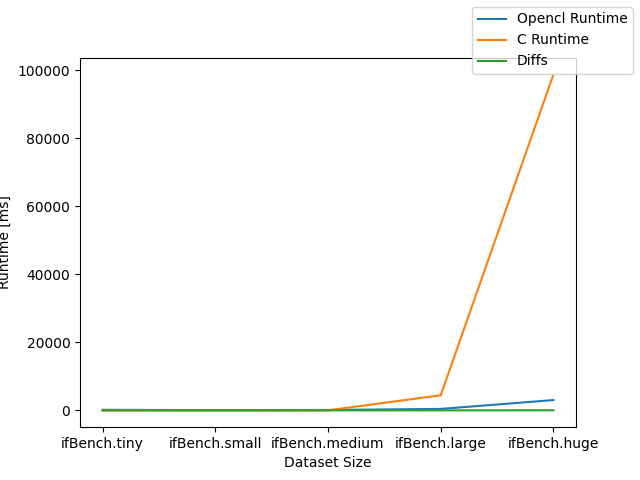
\includegraphics[width=.9\linewidth]{./src/task2.png}
\caption{The performance graphs of benchmarking if then else flattened version}
\end{figure}


\section{Task 3}
\label{sec:orgb2f5188}
I will now try to flatten the following snippet:
\begin{verbatim}
map (\xs is vs -> scatter xs is vs
    ) xss iss vss
\end{verbatim}

Some basic intuition tells me i can still use a scatter. First i have to calculate the indices for
every array after the first one. To do this i could calculate an array of offsets like i calculated
the boolean array in the previous task. Then i can filter that offset array to restore entries with
negative offsets. A rough draft of the transformations is written out below:
\begin{verbatim}
-- Initial data
shape:   [3, 2, 3]
data:    [2, 4, 6, 1, 2, 1, 3, 5]
is:      [2, 1, 0, 0,-1, 2, 1, 0]
-- get the indices
flarr:   [1, 0, 0, 1, 0, 1, 0, 0]
scshp:   [0, 3, 5] -- scan shape arr
flMask:  [0, 0, 0, 3, 3, 5, 5, 5]
-- Now add and filter
is:      [2, 1, 0, 3, 2, 7, 6, 5]
is_fil:  [2, 1, 0, 3,-1, 7, 6, 5]
-- How the scattered data will look
scatter: [6, 4, 2, 1, x, 0, 1, 2]
\end{verbatim}
After the draft, i write up the following more formal syntax

\begin{verbatim}
let flatMap (X_shp, X_dat) (I_shp, I_dat) (V_shp, I_dat) =
  -- The shape arr
  let scanned_shape = scan_exc (+) 0 I_shp
  -- The flag array
  let fl_arr = mkFlagArray I_shp
  let fl_inds= scan (+) 0 fl_arr |> map (\x -> x-1)
  let fl_mask= map (\i -> scanned_shape[i]) fl_inds
  let newI   = map2 (+) I_dat fl_mask
  let filteredI = map (\i -> if I_dat[i] < 0 then -1 else newI[i])
		      (indices I_dat)
  in scatter X_dat I_dat V_dat	      
\end{verbatim}

\section{Task 4}
\label{sec:org19414d6}
Due to time constraints, this was not finished.
\end{document}
